\tikzset{every picture/.style={line width=0.75pt}} 

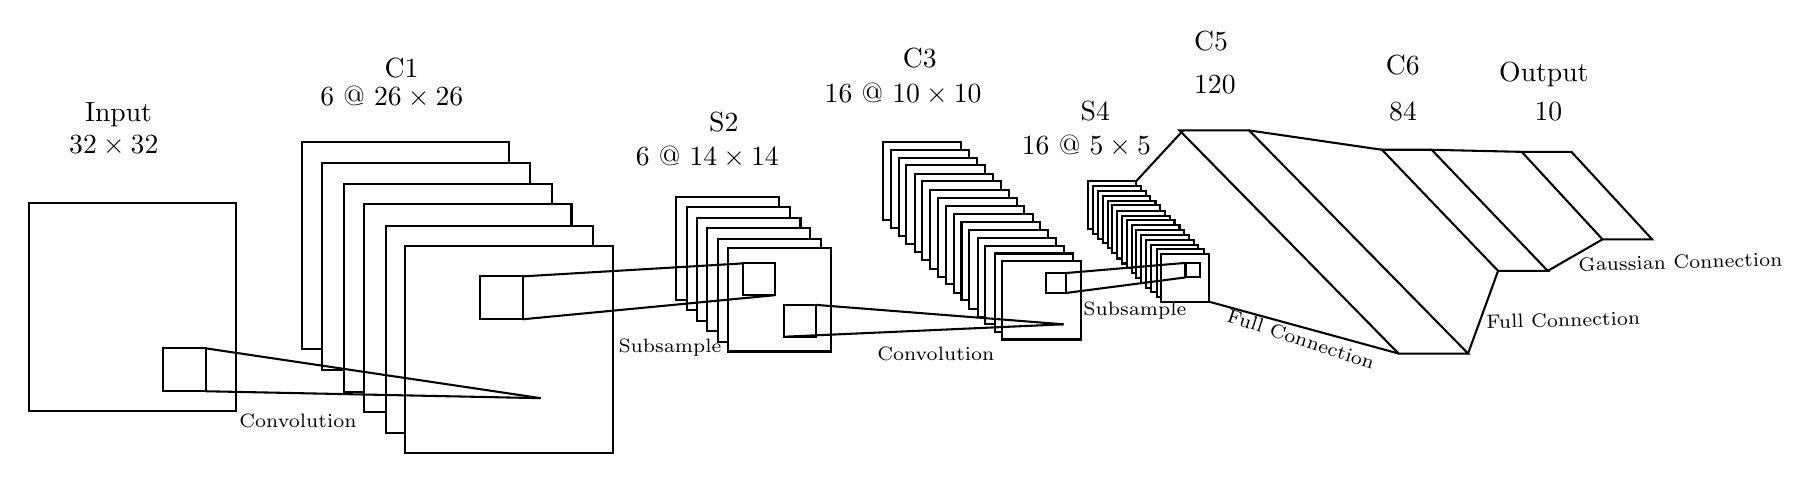
\begin{tikzpicture}[x=0.75pt,y=0.75pt,yscale=-1,xscale=1]

\draw   (19,126) -- (119,126) -- (119,226) -- (19,226) -- cycle ;

\draw  [fill=white   ,fill opacity=1 ] (150.5,96.5) -- (250.5,96.5) -- (250.5,196.5) -- (150.5,196.5) -- cycle ;

\draw  [fill=white   ,fill opacity=1 ] (160.5,106.5) -- (260.5,106.5) -- (260.5,206.5) -- (160.5,206.5) -- cycle ;

\draw  [fill=white   ,fill opacity=1 ] (171,117) -- (271,117) -- (271,217) -- (171,217) -- cycle ;

\draw  [fill=white   ,fill opacity=1 ] (180.5,126.5) -- (280.5,126.5) -- (280.5,226.5) -- (180.5,226.5) -- cycle ;

\draw  [fill=white   ,fill opacity=1 ] (191,137) -- (291,137) -- (291,237) -- (191,237) -- cycle ;

\draw  [fill=white   ,fill opacity=1 ] (200.5,146.5) -- (300.5,146.5) -- (300.5,246.5) -- (200.5,246.5) -- cycle ;

\draw  [fill=white   ,fill opacity=1 ] (191,137) -- (291,137) -- (291,237) -- (191,237) -- cycle ;

\draw  [fill=white   ,fill opacity=1 ] (200.5,146.5) -- (300.5,146.5) -- (300.5,246.5) -- (200.5,246.5) -- cycle ;

\draw  [fill=white   ,fill opacity=1 ] (331,123) -- (380.67,123) -- (380.67,172.67) -- (331,172.67) -- cycle ;

\draw  [fill=white   ,fill opacity=1 ] (335.97,127.97) -- (385.63,127.97) -- (385.63,177.63) -- (335.97,177.63) -- cycle ;

\draw  [fill=white   ,fill opacity=1 ] (341.18,133.18) -- (390.85,133.18) -- (390.85,182.85) -- (341.18,182.85) -- cycle ;

\draw  [fill=white   ,fill opacity=1 ] (345.9,137.9) -- (395.57,137.9) -- (395.57,187.57) -- (345.9,187.57) -- cycle ;

\draw  [fill=white   ,fill opacity=1 ] (351.12,143.12) -- (400.78,143.12) -- (400.78,192.78) -- (351.12,192.78) -- cycle ;

\draw  [fill=white   ,fill opacity=1 ] (355.83,147.83) -- (405.5,147.83) -- (405.5,197.5) -- (355.83,197.5) -- cycle ;

\draw  [fill=white   ,fill opacity=1 ] (351.12,143.12) -- (400.78,143.12) -- (400.78,192.78) -- (351.12,192.78) -- cycle ;

\draw  [fill=white   ,fill opacity=1 ] (355.83,147.83) -- (405.5,147.83) -- (405.5,197.5) -- (355.83,197.5) -- cycle ;

\draw  [fill=white   ,fill opacity=1 ] (430.5,96.5) -- (468.33,96.5) -- (468.33,134.33) -- (430.5,134.33) -- cycle ;

\draw  [fill=white   ,fill opacity=1 ] (434.28,100.28) -- (472.12,100.28) -- (472.12,138.12) -- (434.28,138.12) -- cycle ;

\draw  [fill=white   ,fill opacity=1 ] (438.26,104.26) -- (476.09,104.26) -- (476.09,142.09) -- (438.26,142.09) -- cycle ;

\draw  [fill=white   ,fill opacity=1 ] (441.85,107.85) -- (479.68,107.85) -- (479.68,145.68) -- (441.85,145.68) -- cycle ;

\draw  [fill=white   ,fill opacity=1 ] (445.82,111.82) -- (483.66,111.82) -- (483.66,149.66) -- (445.82,149.66) -- cycle ;

\draw  [fill=white   ,fill opacity=1 ] (449.42,115.42) -- (487.25,115.42) -- (487.25,153.25) -- (449.42,153.25) -- cycle ;

\draw  [fill=white   ,fill opacity=1 ] (445.82,111.82) -- (483.66,111.82) -- (483.66,149.66) -- (445.82,149.66) -- cycle ;

\draw  [fill=white   ,fill opacity=1 ] (449.42,115.42) -- (487.25,115.42) -- (487.25,153.25) -- (449.42,153.25) -- cycle ;

\draw  [fill=white   ,fill opacity=1 ] (453.28,119.78) -- (491.12,119.78) -- (491.12,157.62) -- (453.28,157.62) -- cycle ;

\draw  [fill=white   ,fill opacity=1 ] (457.26,123.76) -- (495.09,123.76) -- (495.09,161.59) -- (457.26,161.59) -- cycle ;

\draw  [fill=white   ,fill opacity=1 ] (460.85,127.35) -- (498.68,127.35) -- (498.68,165.18) -- (460.85,165.18) -- cycle ;

\draw  [fill=white   ,fill opacity=1 ] (464.82,131.32) -- (502.66,131.32) -- (502.66,169.16) -- (464.82,169.16) -- cycle ;

\draw  [fill=white   ,fill opacity=1 ] (468.42,134.92) -- (506.25,134.92) -- (506.25,172.75) -- (468.42,172.75) -- cycle ;

\draw  [fill=white   ,fill opacity=1 ] (464.82,131.32) -- (502.66,131.32) -- (502.66,169.16) -- (464.82,169.16) -- cycle ;

\draw  [fill=white   ,fill opacity=1 ] (468.42,134.92) -- (506.25,134.92) -- (506.25,172.75) -- (468.42,172.75) -- cycle ;

\draw  [fill=white   ,fill opacity=1 ] (472.18,139.02) -- (510.02,139.02) -- (510.02,176.85) -- (472.18,176.85) -- cycle ;

\draw  [fill=white   ,fill opacity=1 ] (476.16,142.99) -- (513.99,142.99) -- (513.99,180.82) -- (476.16,180.82) -- cycle ;

\draw  [fill=white   ,fill opacity=1 ] (479.75,146.58) -- (517.58,146.58) -- (517.58,184.42) -- (479.75,184.42) -- cycle ;

\draw  [fill=white   ,fill opacity=1 ] (476.16,142.99) -- (513.99,142.99) -- (513.99,180.82) -- (476.16,180.82) -- cycle ;

\draw  [fill=white   ,fill opacity=1 ] (479.75,146.58) -- (517.58,146.58) -- (517.58,184.42) -- (479.75,184.42) -- cycle ;

\draw  [fill=white   ,fill opacity=1 ] (484.49,150.32) -- (522.32,150.32) -- (522.32,188.16) -- (484.49,188.16) -- cycle ;

\draw  [fill=white   ,fill opacity=1 ] (488.08,153.92) -- (525.92,153.92) -- (525.92,191.75) -- (488.08,191.75) -- cycle ;

\draw  [fill=white   ,fill opacity=1 ] (484.49,150.32) -- (522.32,150.32) -- (522.32,188.16) -- (484.49,188.16) -- cycle ;

\draw  [fill=white   ,fill opacity=1 ] (488.08,153.92) -- (525.92,153.92) -- (525.92,191.75) -- (488.08,191.75) -- cycle ;

\draw  [fill=white   ,fill opacity=1 ] (529.5,115.5) -- (552.54,115.5) -- (552.54,138.54) -- (529.5,138.54) -- cycle ;

\draw  [fill=white   ,fill opacity=1 ] (531.8,117.8) -- (554.84,117.8) -- (554.84,140.84) -- (531.8,140.84) -- cycle ;

\draw  [fill=white   ,fill opacity=1 ] (534.22,120.22) -- (557.26,120.22) -- (557.26,143.26) -- (534.22,143.26) -- cycle ;

\draw  [fill=white   ,fill opacity=1 ] (536.41,122.41) -- (559.45,122.41) -- (559.45,145.45) -- (536.41,145.45) -- cycle ;

\draw  [fill=white   ,fill opacity=1 ] (538.83,124.83) -- (561.87,124.83) -- (561.87,147.87) -- (538.83,147.87) -- cycle ;

\draw  [fill=white   ,fill opacity=1 ] (541.02,127.02) -- (564.06,127.02) -- (564.06,150.06) -- (541.02,150.06) -- cycle ;

\draw  [fill=white   ,fill opacity=1 ] (538.83,124.83) -- (561.87,124.83) -- (561.87,147.87) -- (538.83,147.87) -- cycle ;

\draw  [fill=white   ,fill opacity=1 ] (541.02,127.02) -- (564.06,127.02) -- (564.06,150.06) -- (541.02,150.06) -- cycle ;

\draw  [fill=white   ,fill opacity=1 ] (543.37,129.68) -- (566.41,129.68) -- (566.41,152.72) -- (543.37,152.72) -- cycle ;

\draw  [fill=white   ,fill opacity=1 ] (545.79,132.1) -- (568.83,132.1) -- (568.83,155.13) -- (545.79,155.13) -- cycle ;

\draw  [fill=white   ,fill opacity=1 ] (547.98,134.29) -- (571.02,134.29) -- (571.02,157.32) -- (547.98,157.32) -- cycle ;

\draw  [fill=white   ,fill opacity=1 ] (550.4,136.7) -- (573.44,136.7) -- (573.44,159.74) -- (550.4,159.74) -- cycle ;

\draw  [fill=white   ,fill opacity=1 ] (552.59,138.89) -- (575.63,138.89) -- (575.63,161.93) -- (552.59,161.93) -- cycle ;

\draw  [fill=white   ,fill opacity=1 ] (550.4,136.7) -- (573.44,136.7) -- (573.44,159.74) -- (550.4,159.74) -- cycle ;

\draw  [fill=white   ,fill opacity=1 ] (552.59,138.89) -- (575.63,138.89) -- (575.63,161.93) -- (552.59,161.93) -- cycle ;

\draw  [fill=white   ,fill opacity=1 ] (554.88,141.39) -- (577.92,141.39) -- (577.92,164.43) -- (554.88,164.43) -- cycle ;

\draw  [fill=white   ,fill opacity=1 ] (557.3,143.81) -- (580.34,143.81) -- (580.34,166.85) -- (557.3,166.85) -- cycle ;

\draw  [fill=white   ,fill opacity=1 ] (559.49,146) -- (582.53,146) -- (582.53,169.03) -- (559.49,169.03) -- cycle ;

\draw  [fill=white   ,fill opacity=1 ] (557.3,143.81) -- (580.34,143.81) -- (580.34,166.85) -- (557.3,166.85) -- cycle ;

\draw  [fill=white   ,fill opacity=1 ] (559.49,146) -- (582.53,146) -- (582.53,169.03) -- (559.49,169.03) -- cycle ;

\draw  [fill=white   ,fill opacity=1 ] (562.38,148.27) -- (585.41,148.27) -- (585.41,171.31) -- (562.38,171.31) -- cycle ;

\draw  [fill=white   ,fill opacity=1 ] (564.56,150.46) -- (587.6,150.46) -- (587.6,173.5) -- (564.56,173.5) -- cycle ;

\draw  [fill=white   ,fill opacity=1 ] (562.38,148.27) -- (585.41,148.27) -- (585.41,171.31) -- (562.38,171.31) -- cycle ;

\draw  [fill=white   ,fill opacity=1 ] (564.56,150.46) -- (587.6,150.46) -- (587.6,173.5) -- (564.56,173.5) -- cycle ;

\draw   (573.47,91) -- (606.96,91) -- (712.48,198.5) -- (678.99,198.5) -- cycle ;

\draw   (83.67,196) -- (104.33,196) -- (104.33,216.67) -- (83.67,216.67) -- cycle ;

\draw    (104.33,196) -- (265.67,220) ;

\draw    (104.33,216.67) -- (265.67,220) ;

\draw   (236.33,161.33) -- (257,161.33) -- (257,182) -- (236.33,182) -- cycle ;

\draw   (363.07,155.07) -- (378.4,155.07) -- (378.4,170.4) -- (363.07,170.4) -- cycle ;

\draw   (383.07,175.07) -- (398.4,175.07) -- (398.4,190.4) -- (383.07,190.4) -- cycle ;

\draw    (257,161.33) -- (363.07,155.07) ;

\draw    (257,182) -- (378.4,170.4) ;

\draw    (517.58,184.42) -- (398.4,175.07) ;

\draw    (517.58,184.42) -- (383.07,190.4) ;

\draw   (509.07,159.73) -- (518.67,159.73) -- (518.67,169.33) -- (509.07,169.33) -- cycle ;

\draw   (576.33,154.83) -- (583.33,154.83) -- (583.33,161.83) -- (576.33,161.83) -- cycle ;

\draw    (576.33,154.83) -- (518.33,159.75) ;

\draw    (576.33,161.83) -- (518.67,169.33) ;

\draw    (575.19,91) -- (552.54,115.5) ;

\draw    (679,198.5) -- (587.6,173.5) ;

\draw   (671.01,100.33) -- (694.94,100.33) -- (750.87,158.67) -- (726.94,158.67) -- cycle ;

\draw    (671.01,100.33) -- (606.96,91) ;

\draw    (726.94,158.67) -- (712.48,198.5) ;

\draw   (738.35,101.33) -- (762.28,101.33) -- (801.17,143.5) -- (777.25,143.5) -- cycle ;

\draw    (738.35,101.33) -- (694.94,100.33) ;

\draw    (777.25,143.5) -- (750.87,158.67) ;

  
\draw (119,226) node [anchor=north west][inner sep=0.75pt]   [align=left] {{\scriptsize Convolution}};
  
\draw (301.67,190) node [anchor=north west][inner sep=0.75pt]   [align=left] {{\scriptsize Subsample}};
  
\draw (426.33,194) node [anchor=north west][inner sep=0.75pt]   [align=left] {{\scriptsize Convolution}};
  
\draw (525.67,172) node [anchor=north west][inner sep=0.75pt]   [align=left] {{\scriptsize Subsample}};
  
\draw (596.9,174.9) node [anchor=north west][inner sep=0.75pt]  [rotate=-18.2] [align=left] {{\scriptsize Full Connection}};
  
\draw (44.67,76.33) node [anchor=north west][inner sep=0.75pt]   [align=left] {Input};
  
\draw (189,54.67) node [anchor=north west][inner sep=0.75pt]   [align=left] {C1};
  
\draw (345.33,81) node [anchor=north west][inner sep=0.75pt]   [align=left] {S2};
  
\draw (524.33,75.67) node [anchor=north west][inner sep=0.75pt]   [align=left] {S4};
  
\draw (438.67,50) node [anchor=north west][inner sep=0.75pt]   [align=left] {C3};
  
\draw (579,42) node [anchor=north west][inner sep=0.75pt]   [align=left] {C5};
  
\draw (671.33,53.67) node [anchor=north west][inner sep=0.75pt]   [align=left] {C6};
  
\draw (37,92) node [anchor=north west][inner sep=0.75pt]    {$32\times 32$};
  
\draw (158,68) node [anchor=north west][inner sep=0.75pt]    {$6\ @\ 26\times 26$};
  
\draw (310,97) node [anchor=north west][inner sep=0.75pt]    {$6\ @\ 14\times 14$};
  
\draw (401,67) node [anchor=north west][inner sep=0.75pt]    {$16\ @\ 10\times 10$};
  
\draw (496,92) node [anchor=north west][inner sep=0.75pt]    {$16\ @\ 5\times 5$};
  
\draw (579,63) node [anchor=north west][inner sep=0.75pt]    {$120$};
  
\draw (719.71,178.58) node [anchor=north west][inner sep=0.75pt]  [rotate=-358.44] [align=left] {{\scriptsize Full Connection}};
  
\draw (673,76) node [anchor=north west][inner sep=0.75pt]    {$84$};
  
\draw (726,56.67) node [anchor=north west][inner sep=0.75pt]   [align=left] {Output};
  
\draw (743,76) node [anchor=north west][inner sep=0.75pt]    {$10$};
  
\draw (764.06,151.08) node [anchor=north west][inner sep=0.75pt]  [rotate=-358.44] [align=left] {{\scriptsize Gaussian Connection}};

\end{tikzpicture}
